\def\hnumber{5}
\def\student{Jerry Sun}
\def\studentid{ys7va}
\documentclass{cs4444}
\usepackage{tikz, pgfplots, graphicx}
\begin{document}

\maketitle

\section{Problem Description}
The goal of this assignment is to write a traditional matrix multiplication program on GPU using CUDA. The experiment is going to be tested on a K20 GPU on artemis node. The primary goal is to optimize the program on GPU using various optimization techniques.

The formula for this matrix multiplication problem is this:

Assume A is of dimension dim1 * dim2, B is of dimension dim2 * dim3, C should be of dimension dim1 * dim3, then:
\[
	\forall 0 < i \leq dim1, 0 < j \leq dim3, C_{ij} = \sum_{k=1}^{dim2} A_{ik} * B_{kj}  
\]
	
Since it is really time consuming to perform a 10000 * 10000 matrix multiplication using CPU, we only test it using a dimension of 3000 * 3000 within the CPU version of the implementation provided. 
	It takes 93.79s to finish.
	
\section{Result Summary}
For $10000 * 10000$ matrices multiplication, my final GPU implementation will take 7.99 seconds in kernel and 9.5 seconds for total runtime, including copy from gloabl memory to device memory. Since I haven't tested the runtime of the CPU version on such a large scale, to make a meaningful comparison, the final optimized version on GPU will only take 0.21420s in kernel execution which is almost 500 times faster then the CPU version. The total runtime is around 1s including memory copy from host to device and device to host. One can expect to see even larger performance gap within a larger problem size.

\section{Metadata}
\subsection{Software}
	SLURM: version 14.11
	
	nvcc: NVIDIA (R) Cuda compiler driver, V8.0.61	
		
\subsection{Hardware}
	GPU: Tesla K20c, detailed specification can be found here:
	
	https://www.nvidia.com/content/PDF/kepler/Tesla-K20-Passive-BD-06455-001-v05.pdf
	
	CPU: 2x16c 32c AMD 6276 with 128 GB RAM
	
\section{Approach}
	For this assignment, it is required to utilize the massive parallelism GPU has to optimize a matrix multiplication problem using CUDA programming model. The general process for this problem works as below:
	\begin{itemize}
		\item malloc necessary memory on device for matrices (both original matrices and result matrieces)
		\item copy two matrices for multiplication from host to device
		\item call kernel method and store the result on device memory allocated in first step
		\item copy the result matrix back onto the host
	\end{itemize}

	In CUDA, it performs its parallelism on two levels, block-level and thread-level. We can consider a thread as a mini-task which are grouped along with other threads in blocks. Blocks are grouped in grids and each block can contain up to 1024 threads (or 512 on older GPUs). Each kernel function will launch on every single threads in parallel if possible. In my implementation, each thread will always be responsible for calculating one single cell in the final output. More specifically, when calling kernel function it needs to pass into two dim3(special variable in cuda) variable to specify the corresponding block and grid size on which the kernel function will launch. Assume, each thread block is a square with T\_block * T\_block number of threads. Then, to handle corner cases in which dimension of matrices are not multiple of T\_block, I use a ceiling function, the result looks like below: 
	
	Note: dim\_1, and dim\_3 is the row \& col number of the final output matrix.
	
	\begin{center}
		dim3 block(T\_block, T\_block);
		
		dim3 grid(dim\_1 - 1) / T\_block + 1, (dim\_3 - 1) / T\_block + 1)	
		
	\end{center}
	 
	After successfully divide the whole task into mini-tasks, the key point then is how to implement the kernel function which can cause huge performance difference. 
	\subsection{Baseline Approach}
		As described above, each thread will be responsible for the computation of one single cell in the final output matrix. The problem we want to figure out then is to retrieve the position of the current thread, since the direct position of the cell relative to the thread in final output matrix can't be directly passed into the kernel function. However,
		 we do have the threadId and blockId as well as the thread/block's dimension prepared inside kernel. Therefore, we can directly map threads onto the matrix, as the position of the threads in the overall grid directly map to the position of the cell in the output matrix.
		 Therefore, we have:
		 
		 r = BlockId.x * BlockDim.x + ThreadId.x
		 
		 c = BlcokId.y * BlockDim.y + ThreadId.y
		 
		 Then the calculation is straightforward as calculating an inner product of one row vector and one column vector:
		 \[
		 C[r][c] = \sum_{i=0}^{dim}A[r][i]B[i][c]
			\]
		
	\subsection{Optimization}
		One can find that the result of the baseline approach is inefficient	from timing result in the next section, since all threads are communicating to the global memory which is super slow. Since each cell in original matrix will be accessed multiple times during calculation, using shared memory in GPU should help. The shared memory in CUDA is shared by a single block, that means as long as one thread in a block loads the value from global memory to shared memory, other threads can also use that value as long as it is in the same block with the original thread. 
		
		Therefore we utilize this fact by dividing the whole matrix into tiles instead of directly calculating the inner product of row and column vectors.
		
		More specifically, the idea of utilizing shared memory works as the image below, Note the image is from Cedric Nugteren.
		\begin{center}
					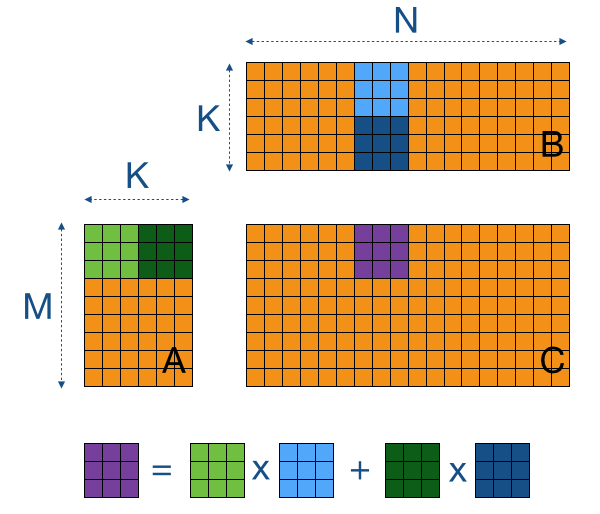
\includegraphics[width=8cm, height=6cm]{gemm2a}
		\end{center}
		We can find that in tiled memory we multiply corresponding tiles at the same time and finally sum all the producst together. 
		
		By doing this, notice that for each block multiplication, each cell in a block is used for multiple times within that block multiplication(more specifically block\_size times). Therefore if we preload two sub matrices into shared memory, the overall performance can be benefitted from increasing number of shared memory accesses.
		
		To implement this, it is important to load the correct block into the shared memory, and also handling corner cases become even trickier. Here to simplify the implementation,  the size of a tile is exactly the size of the block. 
		
		First we need to divide the whole final matrix into tiles(blocks). Then for each block, it needs to find the corresponding rows in Matrix A, and columns in Matrix B and also divide them into N blocks of the same size(as shown in figure1). Then each thread will iterate through N iterations, so that it can get the sum of each block multiplications and place that value in the spot. 
		
		Note, each thread will load exactly two elements from global memory when multiplying two tiles, one is from the element in Matrix A, the other is from element in Matrix B. 
		Also, it is important to synchronize before moving forward into calculation, so that all values are set, otherwise, there might be uninitiated values during calculation.
		
		Further detail implementation can be found directly in code snippets $mult\_matrix\_shared$ in Appendix.
		
		\section{Performance}
	In this section, I will give a brief analysis for the data I retrieved for both versions of kernel function implementations.  For time measurement, I use the \textit{start\_timer} and \textit{stop\_timer} provided in code template. All binary executables are compiled by nvcc using -O3 flag on. For timing, it counts both the total runtime of $computeGPUMMM()$ as well as the kernel function runtime. The block size is set to be 32, unless otherwise specified.	
	 	The program run five times for each number of threads, and I will take the average of that result for further analysis.

\subsection{Runtime data collection}
	Followed are all the timings recorded during testing on Artemis node based on different size of the problem using baseline implementation, and all matrices are assumed to be square matrices. 
	
\begin{table}[ht]
\caption {Baseline with 32 * 32 block}
\centering
\begin{tabular}{c | c c c c c c c c c c}
\hline\hline
dimension(1000*) & 1 & 2 & 3 & 4 & 5 & 6 & 7 & 8 & 9 & 10 \\
\hline
 Kernel & 0.23 & 1.85 & 6.27 & 14.85 & 29.00 & 50.13 & 79.62 & 118.86 & 168.48 & 231.67\\
 Total  & 1.04 & 2.65 & 7.07 & 15.73 & 29.89 & 51.06 & 80.61 & 119.97 & 169.66 & 232.94\\
\end{tabular}
\centering
\end{table}

\begin{table}[ht]
\caption {Shared Memory with 32 * 32 block}
\centering
\begin{tabular}{c | c c c c c c c c c c}
\hline\hline
dimension(1000*) & 1 & 2 & 3 & 4 & 5 & 6 & 7 & 8 & 9 & 10 \\
\hline
 Kernel & 0.01 & 0.06 & 0.22 & 0.48 & 1.02 & 1.73 & 2.78 & 3.87 & 5.93 & 7.99\\
 Total  & 0.73 & 0.87 & 1.03 & 1.29 & 1.91 & 2.63 & 3.83 & 5.00 & 7.13 & 9.49\\
\end{tabular}
\centering
\end{table}

\begin{table}[ht]
\caption {Shared Memory with Different Block Size on 10000 * 10000}
\centering
\begin{tabular}{c| c c c c c c}
\hline\hline
BLOCK\_SIZE & 32 & 16 & 8 & 4 & 2 & 1 \\
\hline
Kernel & 7.99 & 9.68 & 16.92 & 75.27 & 486.55 & 1273.66 \\
Total & 9.49 & 11.02 & 18.17 & 76.58 & 487.82 & 1274.96\\
\end{tabular}
\centering
\end{table}

\begin{center}
\end{center}

\section{Analysis}
From the data above, we can find that the overhead include memory allocation and transferring takes almost a constant time with fixed size problem, and to get a better sense of the comparison within different kernel functions and block size, we will only use kernel runtime for comparison in this section.
\subsection{Shared vs Naive}
\begin{center}
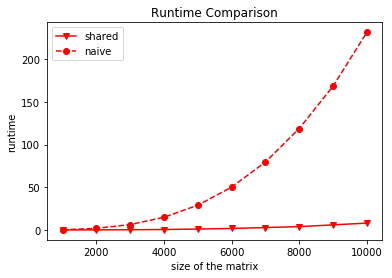
\includegraphics{comparison1}	
\end{center}
The chart above reveals the kernel runtime comparison with between naive and optimized version. We can found a huge performance increase especially with larger size of the matrix. In fact, with a matrix of size 10000 * 10000, the optimized version is indeed about 30 times faster then the unoptimized version. The reason for this kind of speedup is due to the fact that the access speed for shared memory is much faster then the GPU. By loading two corresponding tiles into shared memory, it can effectively reduce the number of accesses to the global memory. In the unoptimized version, with a matrix size of 10000, each element will be loaded 10000 times. However, in the optimized version, the global memory access will be reduced to around 300 (10000/32) times, which causes a huge performance difference.

\subsection{Matrix Size}
\begin{center}
	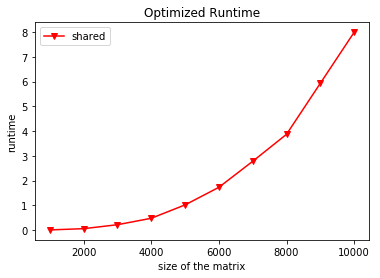
\includegraphics{optimized}
\end{center}
This chart show the runtime of the optimized kernel function with an increasing size of the problem(matrix size). The curve is pretty smooth but has a larger gradient within a larger size, similar to the one in the last figure. This is understandable since a larger problem size will always cause larger overhead other than computing. Especially in this problem, it has fixed block size of 32, then within a larger problem size, it is indeed increasing the number of blocks initiated. As we know, each block in CUDA is assigned to a multiprocessor, and given a relative small, fixed number of multiprocessors, all other blocks are queued. Within a larger queue, and larger data size it is common to find a steeper curve with a larger problem size.

\subsection{Block Size}
\begin{center}
	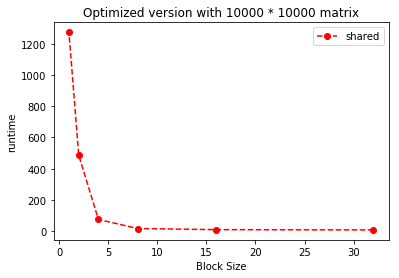
\includegraphics{block}
\end{center}
Then we want to take a look at how different block size might affect the performance. The chart above shows that when block size is small the performance has a huge difference. The reason is that reducing the block size actually reduce the parallelism the device can provide. As discussed earlier, CUDA will initialize all the blocks onto multiprocessors in a queue which is sequential. The parallelism one can get is from huge number of threads running simultaneously in a single block. Therefore, for example, if the block size is only 4 * 4, then it can only compute 16 cells at a time on a single multiprocessor, which is far fewer than the optimal version.

However, one thing worth notice that, using 16 * 16 block doesn't have a huge performance difference than using 32 * 32 block. There are multiple reasons might cause this effect. One major reason is the possible memory bank conflict. Each multiprocessor divided its shared memory into memory banks. Within each memory bank, the access is sequential, that is being said within a single block, only one thread can access one memory bank at a time, all other threads will be put on a queue, which actually sequentialize the whole process. Within a larger number of blocks, it is highly possible to trigger bank conflict if two threads are accessing continuous shared memory. 

\section{Conclusion}
In this assignment, I have gain solid experience in designing and implementing parallel program using CUDA on GPU. The parallel program I implemented shows a substantial performance speedup which only takes less than 9 seconds to finish a size of 10000 * 10000 matrix multiplication problem. The observation made within two versions of kernel function indicates the influence of memory access, like other problems we have countered, is of huge importance is optimizing problem on GPU. 

\section{Finally}
While this has been a harsh semester for me, I did learn a lot in this class especially in those coding assignment. Thanks for this amazing class.
  
\section{Pledge}

\pledge
\newpage
\section{Appendix}
\subsection{matrix\_mult.cu}
\lstinputlisting[language=C]{matrix\_mult.cu}
\subsection{cuda.sh}
\lstinputlisting[language=bash]{cuda.sh}
\section{After All}
However, I have to say, reports are killing me.... 
\end{document}
